\documentclass[12pt, a4paper, notitlepage]{report}
\usepackage{mathptmx}
\usepackage[T1]{fontenc}
\usepackage[utf8x]{inputenc}
\usepackage[english]{babel}
\usepackage{graphicx}
\usepackage{float}
\usepackage{amsmath}
\usepackage{mathtools}
\usepackage{amsfonts}
\usepackage{enumerate}
\usepackage{subfigure}
\usepackage[caption = false]{subfig}
\usepackage[top=2.5cm, bottom=2.5cm, left=2cm, right=2cm]{geometry}
\usepackage[font={small,it}]{caption}
\usepackage{fancyhdr}
\usepackage{listings}
\usepackage{color}

%\graphicspath{ {./Res\_L5\_k10/} {./Res\_L5\_k100/} {./Res\_L5\_k1000/} {./Res\_L10\_k10/} {./Res\_L10\_k100/} {./Res\_L10\_k1000/} {./Res\_L15\_k10/} {./Res\_L15\_k100/} {./Res\_L15\_k1000/} }

\definecolor{dkgreen}{rgb}{0,0.6,0}
\definecolor{gray}{rgb}{0.5,0.5,0.5}
\definecolor{mauve}{rgb}{0.58,0,0.82}
\definecolor{lyellow}{rgb}{1,1,0.9}

\lstset{backgroundcolor=\color{lyellow},
	frame=tb,
	language=Fortran,
	aboveskip=3mm,
	belowskip=3mm,
	showstringspaces=false,
	columns=flexible,
	basicstyle={\small\ttfamily},
	numbers=none,
	numberstyle=\tiny\color{gray},
	keywordstyle=\color{blue},
	commentstyle=\color{dkgreen},
	stringstyle=\color{mauve},
	breaklines=true,
	breakatwhitespace=true,
	tabsize=3
}

\pagestyle{fancy}
\lhead{Tommaso Tabarelli}
\chead{\thepage}
\rhead{\today}
\cfoot{Information theory and computation}
\rfoot{A.y. 2019/2020}
\lfoot{Exercise 7}

\begin{document}

\begin{center}
	\LARGE{Quantum information and computation: homework 7}\\
	\Large{of Tommaso Tabarelli}
\end{center}


\begin{abstract}
	In this homework we are asked to analyze the time development results of the first eigenstate of a \textit{unidimensional quantum harmonic oscillator} subject to a time varying hamiltonian. In particular we are asked to compare results when using different parameters to discretize time (and space). The generation of different results should be done using a fortran program, while the analysis should be made using python and gnuplot scripts.
	To take out the evaluation we are suggested to use fast fourier transforms in fortran executable.
\end{abstract}

\section*{Theory}

The unidimensional quantum harmonic oscillator is the quantum version of the classic harmonic oscillator in which a particle of mass \textit{m} is attached to an extreme of an ideal spring, this one having the other extreme fixed in the origin.

Naming $x$ the spring extension (with respect to the origin), $p$ the particle linear momentum and $k$ the spring constant, the classical system is described by the following equation for the energy:
\begin{equation}
	H = \frac{p^2}{2m} + \frac{1}{2} k x^2
\end{equation}
In the quantum case one should use the corresponding operators:
\begin{equation}
	\hat{H} = \frac{\hat{P}^2}{2m} + \frac{1}{2} k \hat{X}^2
\end{equation}
In our case, the Hamiltonian is the following ($m=1$, $k=1$):
\begin{equation}
H = \frac{\hat{P}^2}{2} + \frac{\left( \hat{X} - X_0(t) \right)^2}{2} 
\end{equation}
where $X_0(t) = t/T$ with $t \in \left[ 0; T\right]$ and $T$ is a parameter.\\

The generic eigenfunction of the quantum harmonic oscillator is:
\begin{equation}
\psi_n (x) = \frac{1}{\sqrt{n! 2^n}} \left( \frac{m \omega}{\pi \hbar} \right)^{1/4} H_n(\xi) e^{-\frac{\xi^2}{2}} \qquad \xi = \sqrt{\frac{m \omega}{\hbar}} x
\end{equation}

We are asked to track the evolution of the first eigenfunction $ ( \hbar = 1, m=1, k=1, \omega = \sqrt{k/m} = 1 ) $:
\begin{equation}
\psi_0 (x) = \frac{1}{\pi^{1/4}} \cdot 1 \cdot e^{-\frac{x^2}{2}} \qquad \xi = x
\end{equation}

The time evolution operator for a given Hamiltonian $H$ acts as following:
\begin{equation}
\vert \psi (x,t\vert t_0) \rangle = \mathbf{U}(t-t_0) \vert \psi_k (x,t_0) \rangle = e^{ -i H(t) (t-t_0)/\hbar } \vert \psi (x, t_0) \rangle
\end{equation}

To evaluate the time evolution the operator has to be expanded as following ($\hbar = 1$, $\frac{\hat{P}^2}{2} = \hat{T}(p)$):
\begin{equation}
e^{ -i \hat{H} \Delta t } \simeq e^{ \frac{-i \hat{V}(x) \Delta t}{2} }  e^{ -i \hat{T}(p) \Delta t } e^{ \frac{-i \hat{V}(x) \Delta t}{2}}
\end{equation}

So to compute the time developing wave function the method is to evaluate it using the following 5 steps (pedices only indicate the step temporary results):
\begin{itemize}
	\item Evaluate
	\begin{equation}
		\psi_1 (x,t) = e^{ \frac{-i \hat{V}(x) \Delta t}{2}} \psi (x,t)
	\end{equation}
	\item Use the Fourier transform:
	\begin{equation}
		\psi_2 (p,t) = \mathcal{F} [\psi_1 (x,t) ]
	\end{equation}
	\item Develop the Fourier transformed wave using the kinetic part of the Hamiltonian operator:
	\begin{equation}
		\psi_3 (p,t) = e^{ -i \hat{T}(p) \Delta t } \psi_2 (p,t)
	\end{equation}
	\item Transform back to $x$ space:
	\begin{equation}
	\psi_4 (x,t) = \mathcal{F}^{-1} [\psi_3 (p,t)]
	\end{equation}
	\item Evaluate
	\begin{equation}
	\psi (x, t + \Delta t) = e^{ \frac{-i \hat{V}(x) \Delta t}{2}} \psi_4 (x,t)
	\end{equation}
\end{itemize}



\section*{Code development}
The Fortran program first reads 4 files in which the parameters are written (space and time intervals limits and number of intervals). Then variables are allocated. After that, the first harmonic oscillator (theoretical) eigenfuntcion ($n = 0$) is calculated on space grid points, then it is time developed following the aforementioned steps (equations (8)-(12)). The Fourier transform is evaluated using some subroutines from the FFTW package (see \textit{http://www.fftw.org}).

All results are stored to proper files.

To handle data analysis in a neater way, a python script was implement. It creates proper folders in which the data is stored, saving current date, time and parameters used during the evaluation as folder name.

The python script also takes care to plot some \textit{.gif} files and images showing the wave function module and its time development. They also compare the "single step evolution" (evaluated using equations (8)-(12)) with the "multi step evolution", which is a single evaluation using $\Delta t = t - t_0 $ (with $t_0 = 0$).

To make compilation and executions faster, some \textit{shell} scripts were also written. 

\section*{Results}

\begin{figure*}[h!]
	\centering
	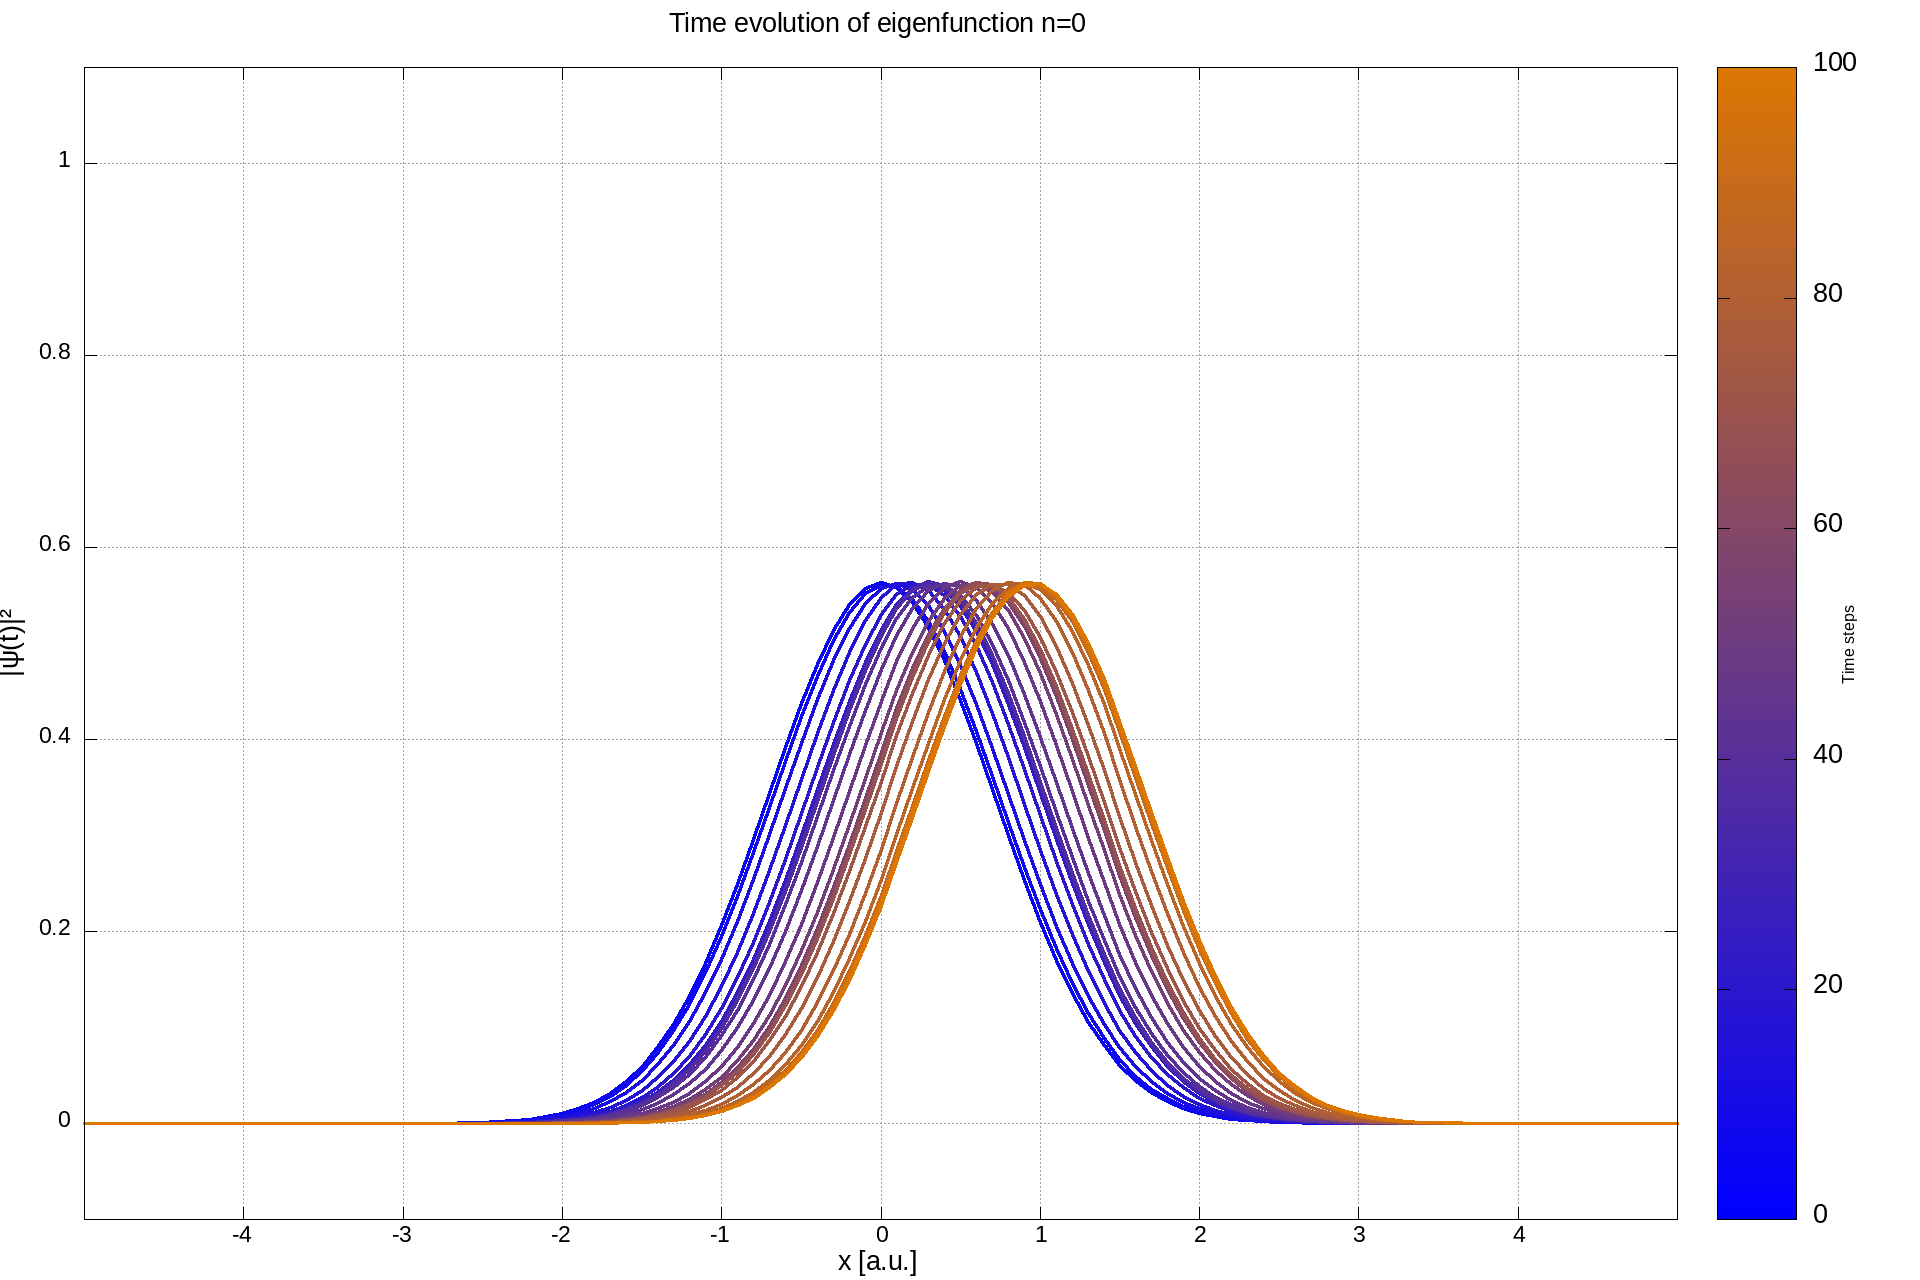
\includegraphics[scale=0.25]{col_t_steps__L5,0_deltax0,1_Ttot20,0_deltat0,2.png}
	\caption{"Time track" of the first harmonic oscillator eigenfunction (n=0) evaluated in [-5,5] using t$\in$[0,20], $\Delta x = 0.1$, $\Delta t = 0.2$.}
\end{figure*}

From the \textit{.gif} files produced by the scripts one can notice that the wave function oscillates when the potential moves. The module of the wave function changes slightly, becoming periodically a bit higher and a bit lower than the starting one. Also, it oscillates in a way similar to that of a classical body in a fixed velocity moving potential.

Since it is a quantum harmonic oscillator system, one should expect that if the potential moves quite fast the function cheanges and becomes that of an excited state, but this behaviour is not observed in this task (even "cheating" changing the maximum potential position, for example using $X_0(t) = V \cdot t/T$ with $V$ "big", say $V=100$, the excited behaviour is not observed, i.e. the wave function does not change its main behaviour). This may be due to the fact that in practice the eigenfunction is developed independently with respect to the system it represents: it does not "know" it should be excited at a certain point because it is not aware the system it came from, making the time evotution as that observed in this task.

\section*{Self-evaluation}
In this task I learned how to evaluate the time evolution of a generic wave function of a quantum system (the  generalization of the method used in this homework is quite straight forward). I also learned how to use \textit{fast Fourier transform} package. Furthermore, I learned how to build \textit{.gif} files to represent in a fancy way a time evolution.

\subsection*{Correctness}

My program does what is expected to do. Some checks are made both in Python script and in Fortran program (for example dimensions are tested to be greater than 0).\\
There are no compilation problems neither memory allocation issues (a special flag is used to compile in order to check for runtime memory errors).\\
Pre- and post-conditions and checkpoints are not used so much due to the large amount of time they require to be implemented (compared to the time we have to do the task).

\subsection*{Stability}

Loops are made only on integers (usually the extreme values of the loop variables are the same used to initialize the dimension of the objects).\\
Sometimes, if the programm is run using "big" parameters values, it can give errors or warnings concerning number representation errors or reading file errors (by gnuplot); anyway, these kind of errors is usually well handled by the programs themselves and it turns out to be not so relevant (the images and the analisys can go on despite them).


\subsection*{Accurate discretization}

Exploring different sets of parameters the following behaviours are observed:
\begin{itemize}
	\item Using too small $\Delta t$ the system in practice does not evolve and even if using big values of $T$ (keeping $\Delta t$ small) it is very slow to go on and develop... On the other side, using too large $\Delta t$ one can notice that the program completely fail in the estimation; to better understand this point, one can use the comparison between the "single step time evolution" and the "multi step time evolution" using the proper file.
	\item One can notice that the $T$ parameter sets the potential shift speed since its vertex always arrive in $x=1$ point, but with different time elongations (using a fixed value for $\Delta t$).
	\item The value of the $\Delta x$ parameter has to be tuned so that the eigenfuntction evaluation through the grid results "quite smooth"; too small values makes the result accurate but require larger computational time and memory, while greater values make risk to make the approximation poor.
	\item The values of the space interval extremes are important to have a good visualization of the function in the images: both too large and too small values lead to a poor visualization.
\end{itemize}

\subsection*{Flexibility}

I tried to comment as much as possible the code so to have a clear and understandable code.

\subsection*{Efficiency}

As aforementioned I did not implemented the \textit{fast Fourier transform} algorithm but I used an alredy implemented package that has been rewarded as one of the fastest evaluation routines (see \textit{http://www.fftw.org}).

To evaluate the theoretical eigenfunction, factorial and Hermite polynomials were needed and so two subroutines were written, but they are quite simple and I think there can be slightly improvements to them.

For what concerns memory and time usage, they depend on the parameters passed. Also, we were asked to use the \textit{fft} because its evaluation is faster than all other methods concerning the use of matrices; for example we could use direct integration evaluating H for every time steps and using it to evaluate the direct tranformation of the wave function, but it would be slower than using fft. \\ \\

My work can be improved: for example, other parameters can be taken as input in Fortran program (for example, mass and $\omega$). Moreover, as aforementioned the max position of the potential can be changed (i.e. added as parameter) to study better the related behaviour and tune better Hamiltonian "velocity" with respect to the total time interval.



\end{document}